\clearpage
\section{Background and concepts}
\label{ch:background}

Esta seção descreve brevemente coceitos e background tais como o paradigma SDN e redes 5G.
%This section briefly introduces background and concepts such as the \acl{SDN} paradigm and the 4G \acl{LTE} networks.

%=============================================================================%
\subsection{Arquitetura hierarquica multi-níveis em Nuvem-Névoa}

A computação em névoa tem como principal objetivo preencher uma lacuna entre a nuvem e os dispositivos finais. Existem várias definições e terminologias na literatura que abordam este paradigma na literatura. Nesta proposta, vamos adotar a definição, o qual é adotado pelo OpenFogConsortium~(OpenFog), publicada pelo \textit{National Institute of Standards and Technology}~(NIST) [1]: 

\begin{displayquote}

"\textit{A computação em névoa é um modelo em camadas para permitir o acesso onipresente a um contínuo compartilhado de recursos de computação escalonáveis. O modelo facilita a implantação de aplicativos e serviços distribuídos com reconhecimento de latência e consiste em nós de névoa (físicos ou virtuais), que residem entre dispositivos finais inteligentes e serviços centralizados (na nuvem)}."

\end{displayquote}
% https://nvlpubs.nist.gov/nistpubs/SpecialPublications/NIST.SP.500-325.pdf. March 2018
% https://www.openfogconsortium.org

Os nós podem ser organizados em arquiteturas multi-níveis - na vertical (para dar suporte ao isolamento), na horizontal (para suportar a federação) ou pela latência entre os nós da \textit{fog} e os usuários finais. A \textit{fog computing} minimiza o tempo de resposta das aplicações suportadas e fornece, para os dispositivos finais, recursos de computação local e, quando necessário, conectividade de rede para serviços centralizados. %Os nós da \textit{fog} são recursos locais que podem ser organizados em arquiteturas multi-níveis e podem ser quaisquer dispositivos que oferece conexão de rede com fio/sem fio com computação, armazenamento e conectividade de rede, como switches, roteadores, smart phones, tablets, laptops, etc. 

\subsubsection{Arquitetura Hierarquica}
Uma arquitetura na névoa verticalmente com N niveis tem como proposito: lidar eficientemente com a quantidade de dados que precisa ser processada e extrair dados significativos para criar mais inteligência em cada nível. Além disso, o número de camadas afeta diretamente o suporte de QoE.
%to deal efficiently with the amount of data that needs to be processed and to extract meaningful data to create more intelligence at each level. Moreover, the number of tiers impacts direclty in the QoE support.
%O OpenFog está assumindo a liderança na padronização de névoa e definiu uma arquitetura de referência que consiste em N camadas de nós, como mostra a Figura~\ref{fig:arch-multi-lvl}

Para fazer isso, primeiro apresentamos uma arquitetura de rede de várias camadas, detalhada na Figura~\ref{fig:arch-multi-lvl}. A camada superior é composta pelos servidores em nuvem que podem ser localizados em um setor público ou privado da nuvem. As nuvens podem ser qualquer provedor de Video sbob Demanda~(VoD), por exemplo, Netflix, Amazon, ou Youtube. Estas nuvem operam o conteudo multimidia original sobre redes WANs. Os 3 níveis seguintes representam a rede fog-cloud organizada hierarquicamente. Este  trabalho leva em consideração os nós da borda com serviços de armazenamento e computação, bem como, é ranqueado de acordo com a área de cobertura de comunicação. Nesse ecossistema multicamada, o Core Network Regional Edge pode gerenciar a coordenação em toda a cidade, por exemplo, unidade de banda de base (BBU) ou provedor de serviços de Internet (ISP). Seguido pela rede de borda de acesso, que suporta algumas dezenas a talvez algumas centenas de nós locais no meio do nevoeiro, por exemplo, estação base ou ponto de acesso. Os gateways de borda podem ser distribuídos em nós de neblina locais, por exemplo, computadores pessoais, laptops e smartphones, onde o nó de neblina retransmite o conteúdo do vídeo por meio de comunicação com ou sem fio. Esses dispositivos têm demandas de tráfego altas e similares, podendo cooperar entre si. Isso pode se conectar a algum tipo de rede local (LAN).

\begin{figure}[htb]
  \centering
  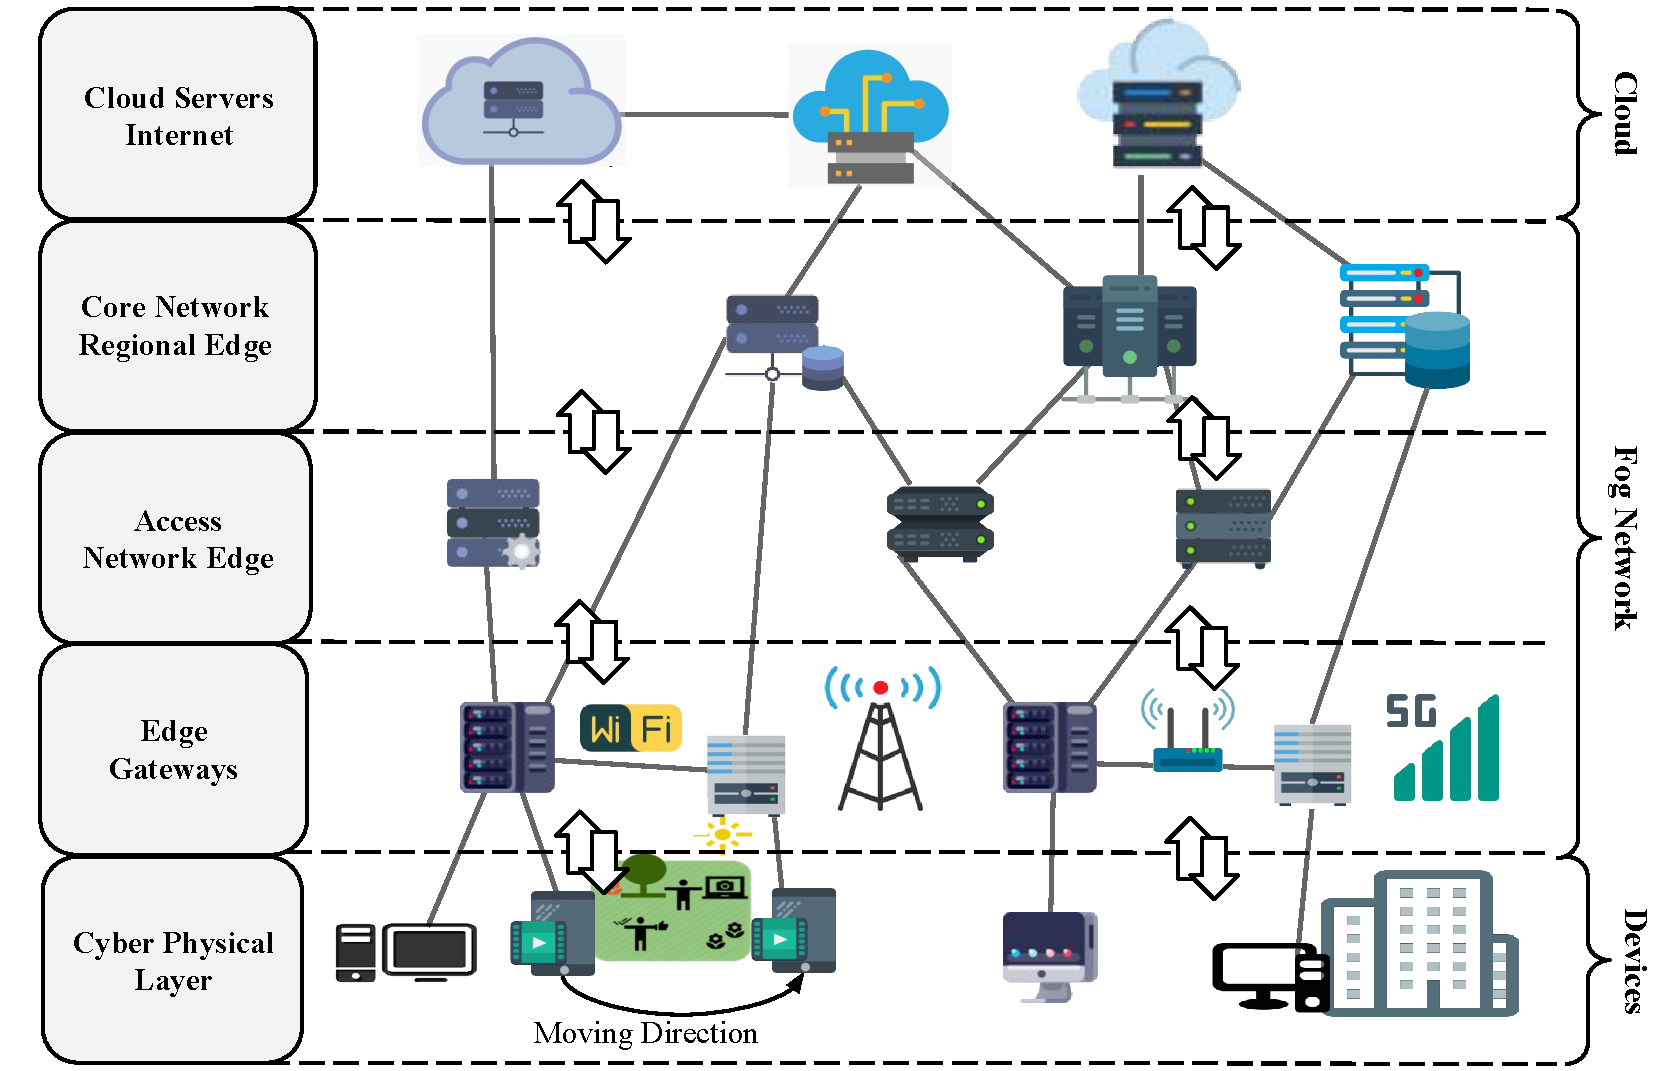
\includegraphics[scale=.5]{arch-multi-lvl}
  \caption{Main components of an multi-lvl environment.}
  \label{fig:arch-multi-lvl}
\end{figure}

Um cenário simples é que um shopping center pode implantar muitos nós de névoa em diferentes andares para fornecer Acesso Wi-Fi e entregar alguns serviços envolvidos (ou seja, navegação interior, distribuição de anúncios, coleções de feedback) para seus clientes. No entanto, no tempo de pico, as capacidades desses nós de nevoeiro não podem servir eficientemente os clientes. Enquanto isso, o provedor de névoa, aqui é o centro comercial, pode estender sua infraestrutura, pagando os recursos de computação e armazenamento terceirizados dos nós de nuvem, que pode ser máquina virtual (VM) alugada de provedores de nuvem em uma base de pay-per-use. Todos os nós de processamento distribuídos (nuvem ou névoa) são gerenciados por um corretor de recursos, que é um componente de gerenciamento de recursos e um planejador para os fluxos de trabalho enviados pelos usuários no lado do nevoa. 
%Neste caso, uma agenda de tarefas, que pode minimizar o tempo de conclusão do fluxo de trabalho, mas corresponde a uma grande quantidade de custo monetário, não é uma solução ideal para fornecedores da fog. 
%Assim, neste artigo, propomos um algoritmo de escalonamento de tarefas que pode conseguir uma boa compensação entre o tempo de execução do fluxo de trabalho e o custo pelo uso dos recursos da nuvem. Os resultados experimentais mostram o excelente desempenho do nosso método comparado com alguns outros trabalhos.	

%-----------------------------------------------------------------------------%
\subsection{HTTP Adaptative Streaming and MPEG-DASG standard}
\label{sec:has-dash}

As aplicações de video streaming baseadas em MPEG-DASH, a technology that dynamically adapts to changing network conditions by requesting content in chunks encoded at different bitrates, and which is used by major streaming services like Netflix and YouTube.
%In this proposal, we focus on video streaming applications based on MPEG-DASH (Dynamic Adaptive Streaming over HTTP), a technology that dynamically adapts to changing network conditions by requesting content in chunks encoded at different bitrates, and which is used by major streaming services like Netflix and YouTube.
There are several key benefits in the adaption of this new standard. Due to the fact that several major media companies took part in its development, the new protocol will eliminate technical issues in delivery and compression. In essence, it aims to combine all of the technologies and standards into one, making streaming support seamless on all devices. In turn, it aims to reduce technical headaches and transcoding costs. Content publishers can generate a single set of files for encoding and streaming that should be compatible with as many devices as possible, from mobile to OTT, as well as to the desktop via plug-ins or HTML5. Consumers will not have to worry about whether their devices will be able to play the content they want to watch.

\begin{figure}[htb]
  \centering
  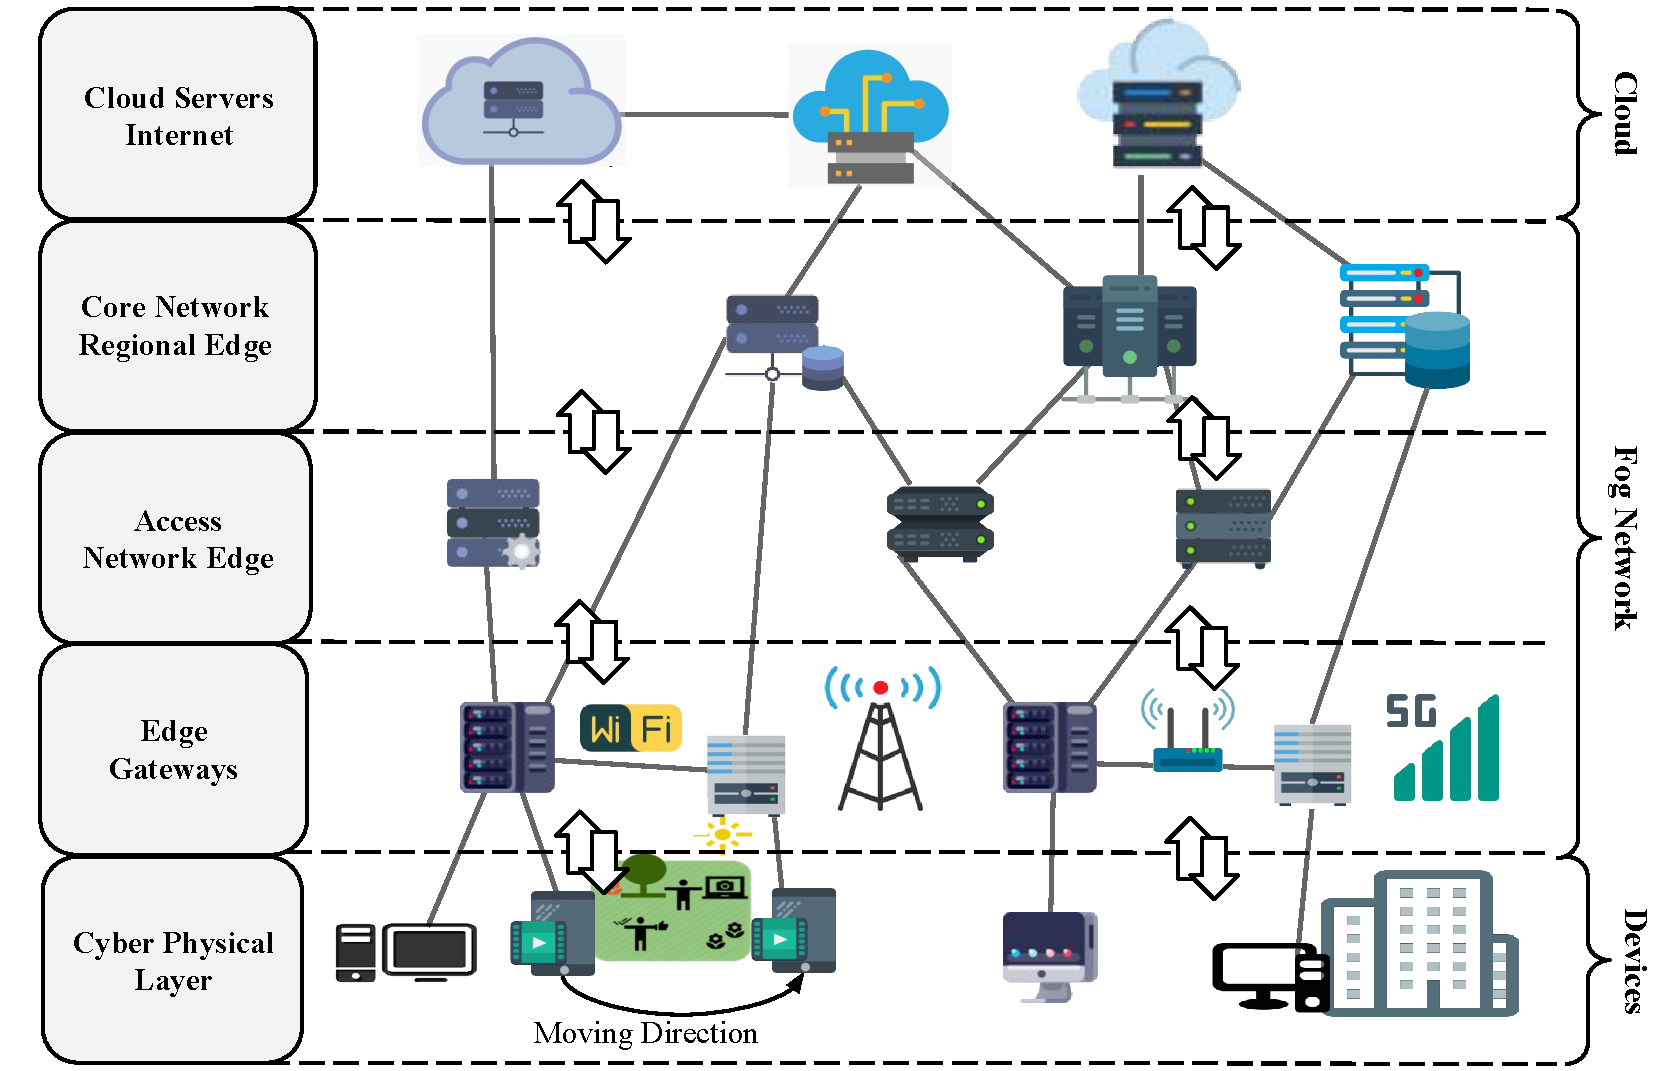
\includegraphics[scale=.5]{arch-multi-lvl}
  \caption{Main components of an multi-lvl environment.}
  \label{fig:arch-multi-lvl}
\end{figure}


By parsing the MPD, the DASH client learns about the program timing, media-content availability, media types, resolutions, minimum and maximum bandwidths, and the existence of various encoded alternatives of multimedia components, accessibility features and required digital rights management (DRM), media-component locations on the network, and other content characteristics. 

Out of Scope
The MPEG-DASH specification only defines the MPD and the segment formats. The delivery of the MPD and the media encoding formats containing the segments, as well as the client behavior for fetching, adaptation heuristics, and playing content, are outside of MPEG-DASH’s scope.


%-----------------------------------------------------------------------------%
\subsubsection{Arquitetura Hierarquica para Bitrate Schemes}
\label{subsec:bitrate-schemes}

%Implementing a multi-tier architecture has a dual purpose: to deal efficiently with the amount
%of data that needs to be processed and to extract meaningful data to create more intelligence at
%each level. Moreover, the number of tiers impacts direclty in the QoE support.

Each ABR scheme proposes many criteria for bitrate decisions, where they work only under
indirect or implicit assumptions and specific scenarios, and focuses on a specific deployment or
different network characteristics. Currently, there is a lack of a general consistent framework
that can formally evaluate and compare different bitrate adaptation schemes, and test and
verify the efficiency of their components. To the best of our knowledge, only a few algorithms
formally describe what objective they want to optimize, and thus, it is challenging to make
an effective comparison.

In this part, we provide a feature comparison between various state-of-the-art bitrate
adaptation schemes, and are available in terms os the following aspects:

\begin{itemize}

\item Heurisic:	

\item Fairness:

\item \ac{QoE}:

\item \ac{QoE} optimization:

\item Number of Clients:

\item Content type:

\item Heterogeneity:

\item SVC support: Does the adaptation algorithm support the streaming of SVC-encoded video?

\item BG Traffic: Does the paper include background traffic in their experimental tests?

\end{itemize}

\subsubsection{Fatores de influencia no QoE}

% Quality Improvement for HTTP Adaptive Streaming over Mobile Networks Hung Thai Le
\begin{itemize}

\item Delay inicial

\item Interrupçoes duração

\item interrupções frequencia

\item Amplitude qualidade 

\item troca de qualidade

\item latencia ao vivo 

\end{itemize}